\documentclass{article}
\author{Wenzhao Xu, Haoyan Cai}
\title{STAT 542 Final Project Proposal}
\usepackage{amsmath}
\usepackage{graphicx}
\usepackage{subfig}
\usepackage{multirow}
\usepackage[top=1in, bottom=1in, left=1.25in, right=1.25in]{geometry}

\begin{document}
	\maketitle
	
	\section{Introduction} % (fold)
	\label{sec:introduction}
	
	\paragraph{} The data are about accelerometer data from mobile device. The train data contain X,Y,Z acceleration data from 387 devices and testing data set have 90024 testing sequences. In addition, for each test sequence, we have information of a possible device. The goal is to judge whether this possible device is the true device that generate the test sequ ence. 
	
	% section introduction (end)
	
	\section{Data Set} % (fold)
	\label{sec:section_name}
	Package "ff" is used to extract data from a large csv file and unix time is converted to GMT time. There are totally 387 training devices, and 90024 testing sequences. A typical visulization of data is shown in Figure 1, in which Device 7 is a device with long sampling time and total 523187 points while Device 770 has limited sampling points as 28475.
	\begin{figure}
		\centering
		\subfloat[Device 770]{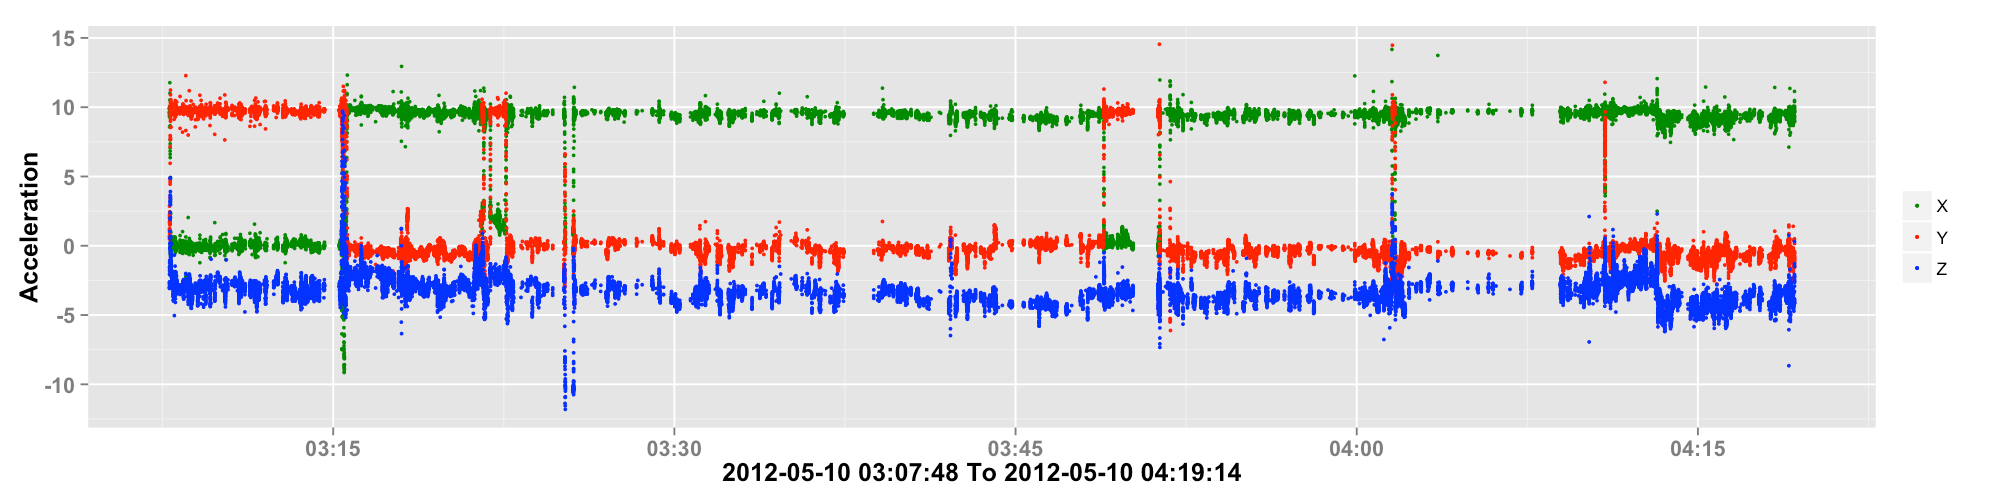
\includegraphics[width=1\textwidth]{770.png}}\\
		\subfloat[Device 7]{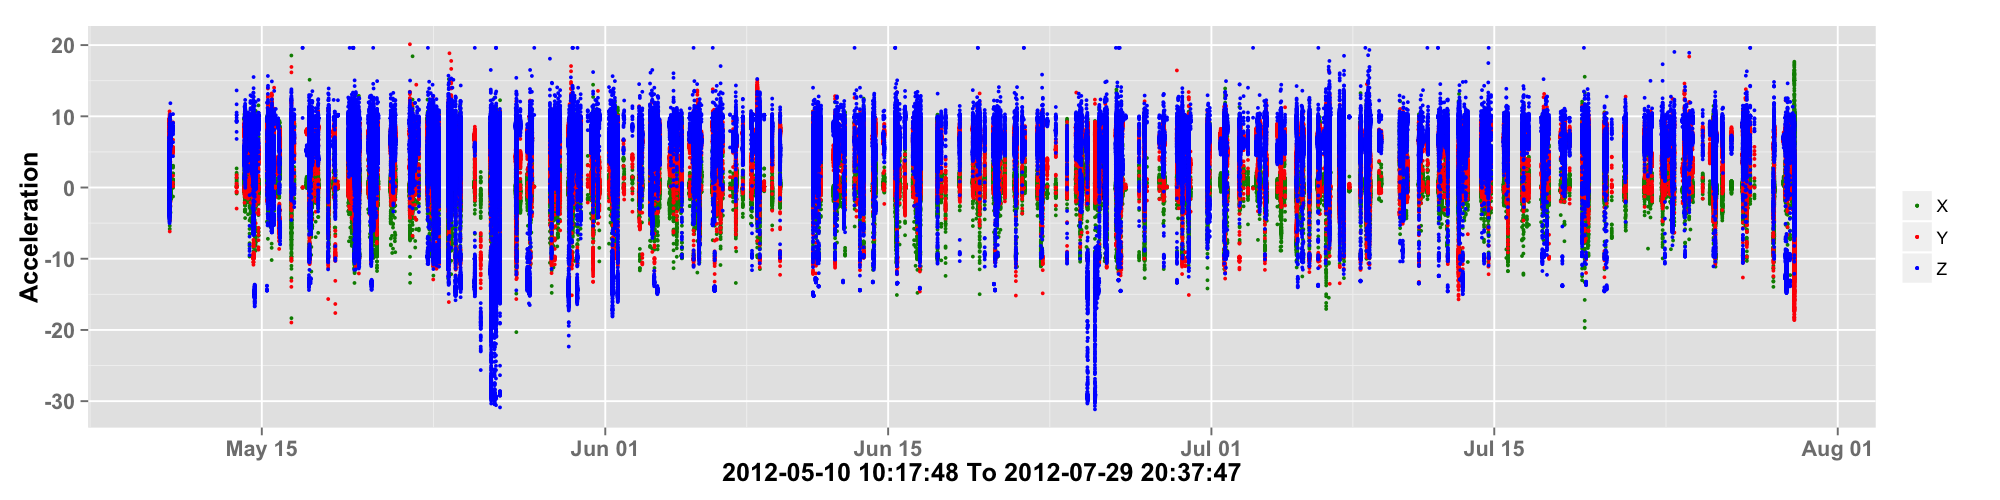
\includegraphics[width=1\textwidth]{7.png}} \\
		\caption{Acceleration Data Along Time}
	\end{figure}
	
	\paragraph{}In test data, we need to identify the professed device is the true number. Figure 2 shows two sequence whose professed device is 770. Compared with the train data with device 770, it seems sequence 838966 is likely belong to Device 770 while sequence 690194 is not since the range of X,Y,Z in sequence 838966 is in consistnace with training data of device 770. 
	\begin{figure}
		\centering
		\subfloat[Sequence 690194]{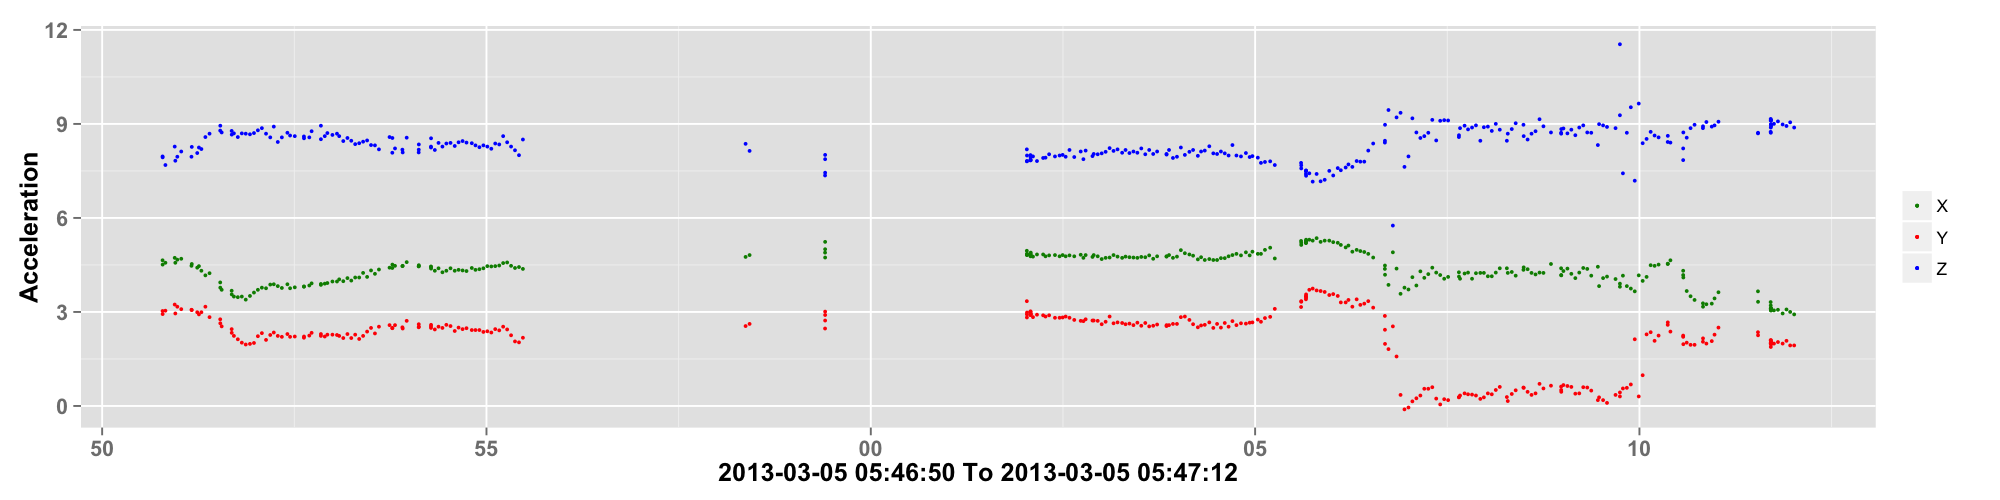
\includegraphics[width=1\textwidth]{690194.png}}\\
		\subfloat[Sequence 838966]{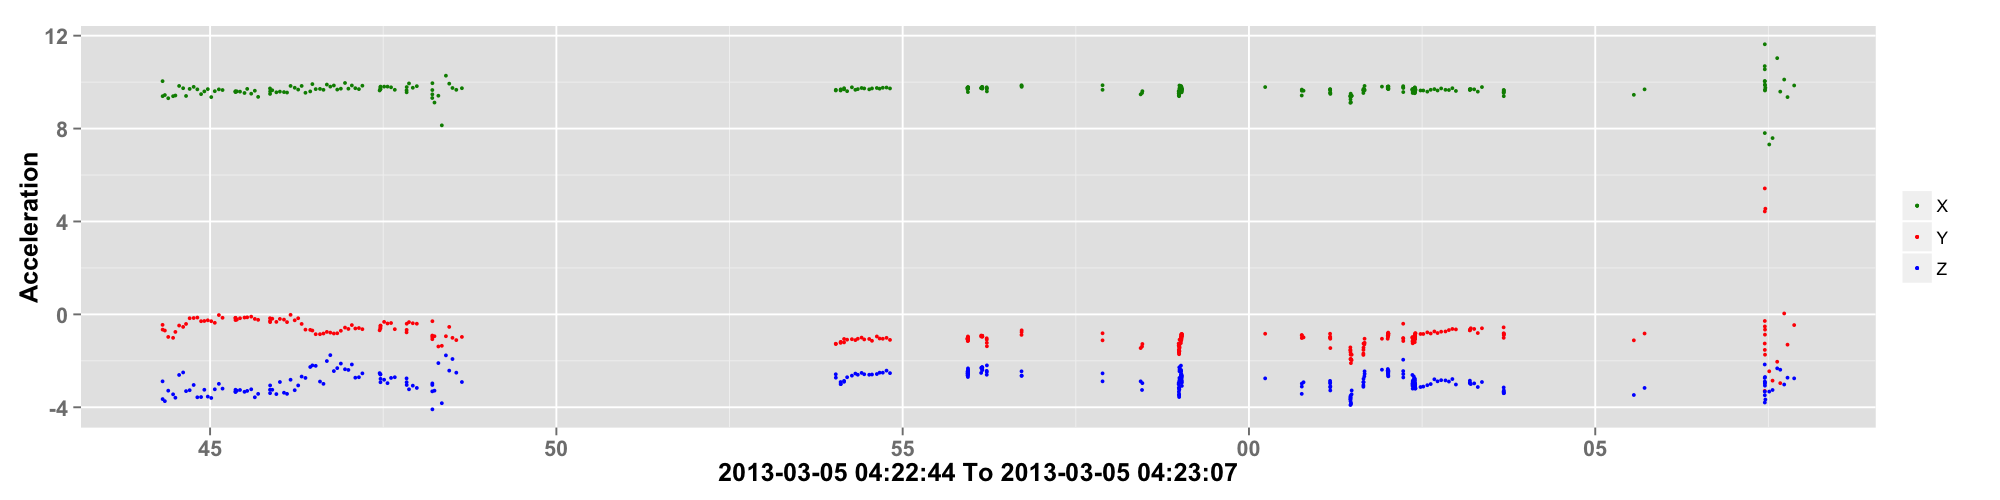
\includegraphics[width=1\textwidth]{838966.png}}
		\caption{Test Sequence with Professed Device as 770}
	\end{figure}
	
	% section section_name (end)
	

	
	\section{Potential Approach} % (fold)
	\label{sec:potential_approach}
	\paragraph{}The data involve time dimension, which is a very important feature. Since we can't use the data leakage such as sampling frequencies of devices, we plan to use following methods:
	
	
	\paragraph{} First, we need to extract the features from the raw data file such as the range of X,Y,Z, the difference between X and Y, between X and Z, and between Y and Z, autocorrelation of X,Y and Z, correlations between X,Y and Z.  Time series analysis 
	
	
	\paragraph{} One of the big problem is that how can we define the probability of been rejected. 
	\begin{itemize}
		\item Method1: Using 
		\item Method2:
		\item ......
	\end{itemize}
	
	
	
	% section potential_approach (end)
	
\end{document}




